\documentclass[parskip=full]{scrartcl}

\pdfoutput=1

\title{Small Data Oversampling  \\ \LARGE{Improving small data prediction accuracy using the Geometric SMOTE algorithm}}

\author{
	Georgios Douzas\(^{1}\), Fernando Bacao\(^{1}\), Maria Lechleitner\(^{1*}\) 
	\\
	\small{\(^{1}\)NOVA Information Management School, Universidade Nova de Lisboa}
	\\
	\small{*Corresponding Author}
	\\
	\\
	\small{Postal Address: NOVA Information Management School, Campus de Campolide, 1070-312 Lisboa, Portugal}
	\\
	\small{Telephone: +351 21 382 8610}
}

\usepackage{breakcites}
\usepackage{float}
\usepackage{graphicx}
\usepackage{geometry}
\usepackage[colorinlistoftodos]{todonotes}
\geometry{
	a4paper,
	total={170mm,257mm},
	left=18mm,
	right=18mm,
	top=18mm,
}
\usepackage{amsmath}
\newcommand{\inlineeqnum}{\refstepcounter{equation}~~\mbox{(\theequation)}}
\usepackage{enumitem}
\usepackage[ruled,vlined]{algorithm2e}
\usepackage{booktabs}
\usepackage{pgfplotstable}
\pgfplotsset{compat=1.14}
\usepackage{longtable}
\usepackage{tabu}
\usepackage{hyperref}
\usepackage{csvsimple}
\usepackage{graphicx}
\usepackage{adjustbox}
\usepackage{longtable}
\usepackage{caption}
\date{}

\begin{document}

\maketitle

\begin{abstract}
In the age of the data deluge there are still many domains and applications
restricted to the use of small datasets. The ability to harness these small
datasets to solve problems through the use of supervised learning methods can
have a significant impact in many important areas. The insufficient size of data
sets usually results in unsatisfactory performance of machine learning
algorithms. The current research work aims to contribute to mitigate the small
dataset problem through the creation of artificial instances, which are added to
the training process. The over-sampling algorithm Geometric SMOTE is applied to
generate new instances and enhance the initial dataset. Experimental results
show a significant improvement in accuracy when compared with the use of the
original small dataset and also over other over-sampling techniques such as
Random Oversampling, SMOTE and Borderline SMOTE. These findings show that
over-sampling research, developed in the context of imbalanced learning, can
also be a valid option to improve accuracy in small data problems.
\end{abstract}

\section{Introduction}
Insufficient size of data sets is a common issue in many supervised learning
tasks \cite{Niyogi.1998}, \cite{AbdulLateh.2017}. The limited availability of
training samples can be caused by different factors. First, data is becoming an
increasingly expensive resource \cite{Li.2007} as the process to retain them is
getting more complex due to strict privacy regulations such as the General Data
Protection Regulation (GDPR) \cite{EuropeanCommission.2019}. Additionally, the
small dataset problem can be found in numerous industries where organizations
simply do not have access to a reasonable amount of data. For example,
manufacturing industries are usually dealing with small number of samples in
early stages of product developments and health care organizations have to work
with different kinds of rare diseases, where very few records are available
\cite{AbdulLateh.2017}.

In machine learning, researchers are usually concerned with the design of
sophisticated learning algorithms when aiming to improve prediction performance.
However, increasing the sample size is often a more effective approach. A rule
of thumb is that "a dumb algorithm with lots and lots of data beats a clever one
with modest amounts of it" \cite{Domingos.2012}. Generally, small training
samples are characterized by a loose data structure with multiple information
gaps. This lack of information negatively impacts the performance of machine
learning algorithms \cite{Lin.2018}. Consequently, the knowledge gained from
models trained with small sample sizes is considered unreliable as well as
imprecise and does not lead to a robust performance \cite{AbdulLateh.2017}.

Considering the size of data, there are two types of problems: First, the
insufficiency of data belonging to one class (imbalance learning problem) for a
binary or multi-class classification task and second, the size of the whole
dataset (small dataset problem) for any classification or regression task
\cite{Sezer.2014}. In both cases, small training samples affect the performance
of machine learning models \cite{Tsai.2008}. A theoretical definition of "small"
can be found in statistical learning theory by Vapnik. A sample size is defined
as small, if the ratio between the number of training samples and
Vapnik-Chervonenkis (VC) dimensions is approximately less than 20. VC dimensions
are determined as the maximum number of vectors that can be separated into two
classes in all possible ways by a set of functions \cite{Vapnik.2008}.

Under-representation of observations in the sample set can be solved in
different ways. The use of synthetic data derived from existing observations is
a promising approach to the problem \cite{Sezer.2014}. Techniques to
artificially add information by extending the sample size, and eventually
improving the performance of the algorithms, can translate into significant
improvements in many application domains. However, it is important to note that
the challenge in artificial data generation is to create data which extend the
training set without creating noise \cite{Li.2006}. Additionally, generating
artificial data will only work if the initial sample is representative of the
underlying population. Figure \ref{fig:relationship} shows the relationship
between population, sample and synthetic data.

\begin{figure}[H]
	\centering
	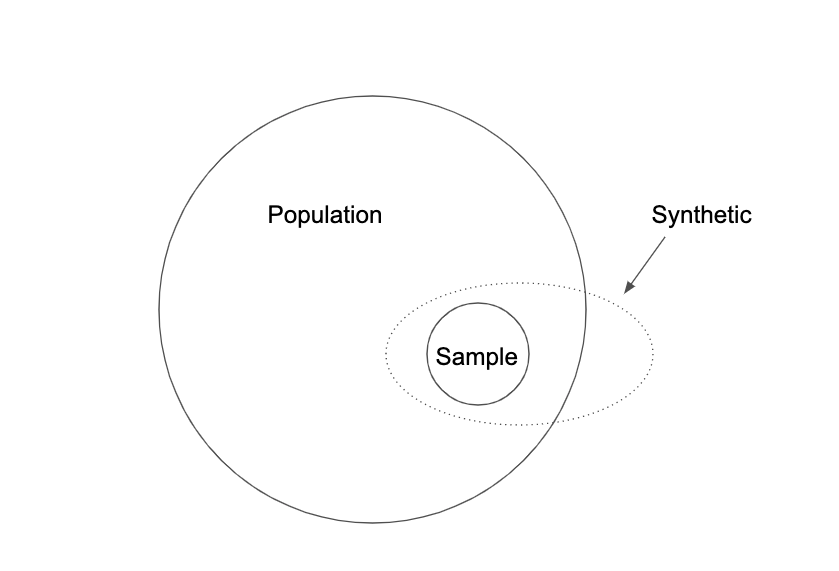
\includegraphics[width=0.60\linewidth]{../analysis/relationship.png}
	\caption{Relationship between population, sample and synthetic data \cite{Li.2006}.}
	\label{fig:relationship}
\end{figure}

The next sections will describe an effective way to tackle the small dataset
problem. In chapter 2, the previously studied solutions are reviewed. A detailed
description of the proposed method is presented in chapter 3. This is followed
by the research methodology and the experimental results in chapters 4 and 5.
Finally, the paper is concluded with an analysis of the experimental results in
chapter 6.

\section{Related work}

Several data pre-processing methods to increase the data size have been
presented by the research community. In this section, the most important
approaches are reviewed and the state-of-the-art to improve small dataset
learning is reported. We start by describing fuzzy theories, which have
historically been the most used approach to mitigate the small dataset problem.
Next, we look at re-sampling mechanisms, which mainly consist of bootstrapping
techniques, and finally, we review over-sampling methods, developed in the
context of imbalanced learning, that can be a valuable option to increase the
sample size in small datasets.

\subsection{Fuzzy theories}

Many artificial sample generation techniques presented in the literature are
based on fuzzy theories \cite{AbdulLateh.2017}. The fuzzy set theory defines a
strict mathematical framework to generalize the classical notion of a dataset,
providing a wide scope of applicability, especially in the fields of information
processing and pattern classification \cite{Zimmermann.2010}. Based on this
concept, several methods have emerged in the last decade to estimate or
approximate functions which are generating artificial samples for small data
sets.

The fundamental concept of creating synthetic data is called Virtual Sample
Generation (VSG) and was originally proposed by \cite{Niyogi.1998}. The idea is
to create additional observations based on the current set of examples by using
prior information. The introduction of virtual examples expands the effective
training set size and can therefore help to mitigate the learning problem.
\cite{Niyogi.1998} showed that the process of creating artificial samples is
mathematically equivalent to incorporating prior knowledge. They demonstrated
the concept on object recognition by mathematically transforming the views of
3D-objects and therefore generating artificial samples.

Based on the above approach, several closely related studies were developed for
manufacturing environments. The first method to overcome scheduling problems due
to the lack of data in early stages of manufacturing systems was the creation of
a Functional Virtual Population (FVP) \cite{Li.2003}. The idea was to create a
number of synthetic samples within a newly defined domain range. Although, the
process was manually configured, its application dramatically improved the
classification accuracy of a neural network. 

\cite{Huang.2004} proposed the Diffusion-Neural-Network (DNN) method, an
approach that fuzzifies information in order to extend a small dataset. It
combines the principle of information diffusion by \cite{Huang.1997} with
traditional Neural Networks to approximate functions. The information diffusion
method partially fills the information gaps by using fuzzy theories to represent
the similarities between samples and subsequently derive new ones.

In order to fully fill the information gaps, Mega-Trend-Diffusion (MTD)
\cite{Li.2007} combines data trend estimation with a diffusion technique to
estimate the domain range, thus avoiding over-estimation. It diffuses a set of
data instead of each sample individually. It is considered as an improvement of
DNN and was initially developed to improve early flexible manufacturing system
scheduling accuracy. In further research, MTD is widely used as a synthetic
sample generation method and is recognized as an effective way to deal with
small dataset problems \cite{AbdulLateh.2017}.

MTD only considers the data for independent attributes and does not deal with
their relationships. Genetic Algorithm Based Virtual Sample Generation was
proposed that takes the relationship among the attributes into account and
explores the integrated effects of attributes instead of dealing with them
individually. The algorithm has three steps: Initially, samples are randomly
selected to determine the range of each attribute by using MTD functions. Next,
a Genetic Algorithm is applied to find the most feasible virtual samples.
Finally, the average error of these new samples is calculated. The results
outperformed the ones using MTD and also showed better performance in prediction
than in the case of no generation of synthetic samples \cite{Li.2014}.

\subsection{Random over-sampling}

An alternative approach to fuzzy theories as well the most well-known artificial
sample generation method is the Bootstrapping Procedure \cite{AbdulLateh.2017}
or Random Over-Sampling (ROS) as is known in the imbalanced learning research
area. The main difference to the previously presented techniques is that ROS
creates expands the training set by re-sampling instances from the original
dataset with replacement \cite{Efron.1993}. Therefore, it allows the algorithms
to use the same sample more than one time to gradually revise the identified
patterns in order to improve predictive accuracy. However, ROS may cause
over-fitting when applied to small data because it repetitively uses the same
information \cite{Tsai.2015}, \cite{Li.2018}. Nevertheless, \cite{Ivanescu.2006}
applied ROS in batch process industries where it was shown that it may help
mitigate the small data problem.

\subsection{Informed over-sampling}

A different approach to fill information gaps is informed over-sampling. It is
an artificial data generation strategy originally developed in the context of
machine learning to deal with the imbalanced learning problem. Therefore, its
origin comes from a different research community than the fuzzy and re-sampling
strategies presented above. Although the small data and imbalanced learning
problems are similar, it seems that their proposed solutions had very few
connections so far.

In the imbalanced learning problem, the classes of the given dataset are
significantly skewed i.e. the dataset has a large number of observations in one
of the classes, called majority class, and a relatively small number of
observations in the other class(es), called minority class(es). This constitutes
a problem for the learning phase of the algorithm resulting in low accuracy for
the minority class(es). In practice, the imbalanced dataset problem is very
common issue in supervised learning. Especially, in the fields of fraud
detection, product categorization and disease diagnosis, an imbalanced dataset
is the norm rather than the exception \cite{He.2013}.

\subsubsection{SMOTE}

There are several methods presented in the literature that belong in the
over-sampling category. The first method to be  proposed and still the most
popular is the Synthetic Minority Oversampling TEchnique (SMOTE). SMOTE is based
on the idea of \( k \)-nearest neighbors and linear interpolation as a data
generation mechanism. More specifically, SMOTE proposes to form a line segment
between neighboring minority class instances and generate synthetic data between
them \cite{Chawla.2002}. The algorithm is very popular due to its simplicity as
well as its robustness. Numerous variations have been proposed based on SMOTE,
increasing its status as the staple idea in over-sampling for imbalanced
learning problems \cite{Fernandez.2018}. However, SMOTE has some significant
limitations when it comes to the sample generation process. In practice, the
separation between majority and minority class areas is often not clearly
definable. Thus, noisy samples may be generated when a minority sample lies in
the region of the majority classes. Figure \ref{fig:noisy-examples} presents a
scenario where a minority instance is generated within the majority region
(noisy sample).

\begin{figure}[H]
	\centering
	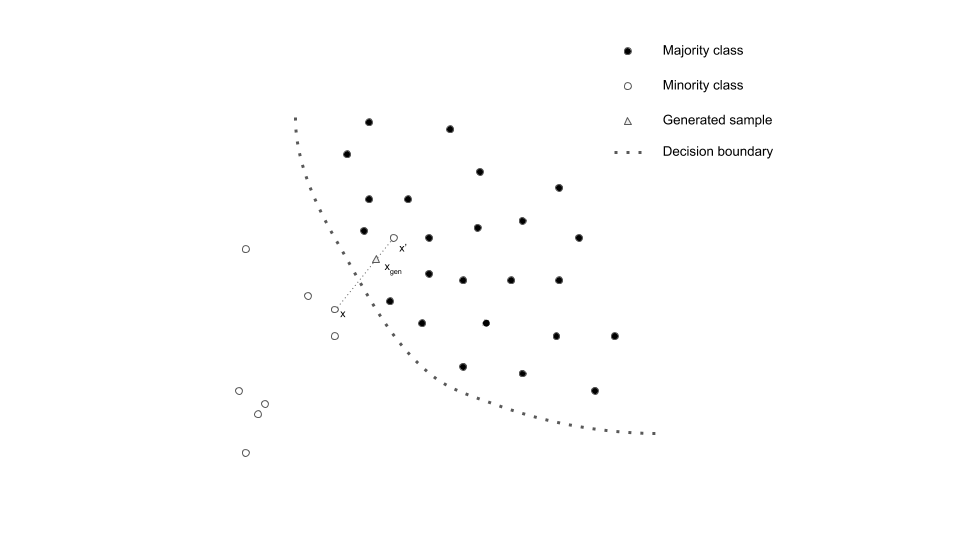
\includegraphics[width=1.0\linewidth]{../analysis/noisy_examples.png}
	\caption{Generation of noisy examples.}
	\label{fig:noisy-examples}
\end{figure}

Furthermore, redundant instances may be generated within dense minority regions,
as so that they do not add any relevant information to the classifier and may
lead to over-fitting. Figure \ref{fig:redundant-examples} demonstrates an
example where a minority  class instance is generated in a dense minority class.
This new observation belongs to the same dense cluster as the original and is
therefore less useful. 

\begin{figure}[H]
	\centering
	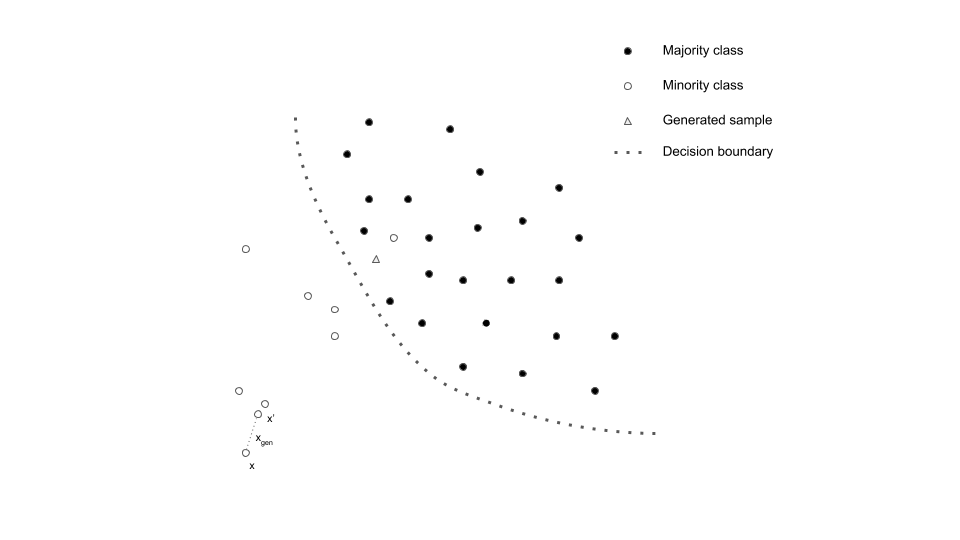
\includegraphics[width=1.0\linewidth]{../analysis/redundant_examples.png}
	\caption{Generation of redundant examples.}
	\label{fig:redundant-examples}
\end{figure}

Although SMOTE is recognized as an over-sampling technique for imbalanced
datasets, it can also be used for solving the small dataset problem.
\cite{Li.2018} showed that SMOTE is able to successfully fill the information
gaps with synthetic samples. However, given its limitations, SMOTE did not
achieve the best results within their study.

\subsubsection{G-SMOTE}

The novel data generation procedure Geometric SMOTE (G-SMOTE) has been presented
with the objective to improve the above mentioned limitations of the SMOTE
algorithm \cite{Douzas.2019}. G-SMOTE can be seen as a substitute of SMOTE,
enhanced by geometric properties. Compared to SMOTE, it expands the data
generation area and prevents the creation of noise. Instead of connecting a
minority sample and one of its minority class nearest neighbors with a line
segment, the instances are generated in a geometrical region around the minority
sample. Furthermore, G-SMOTE is designed to avoid the generation of noisy
samples by introducing the \textit{selection strategy} hyper-parameter. Figure
\ref{fig:smotevsgsmote} demonstrates the distribution of artificially created
samples by SMOTE versus G-SMOTE. Increasing number of \( k \) neighbors, SMOTE
tends to generate noisy samples, whereas G-SMOTE avoids this scenario.

\begin{figure}[H]
	\centering
	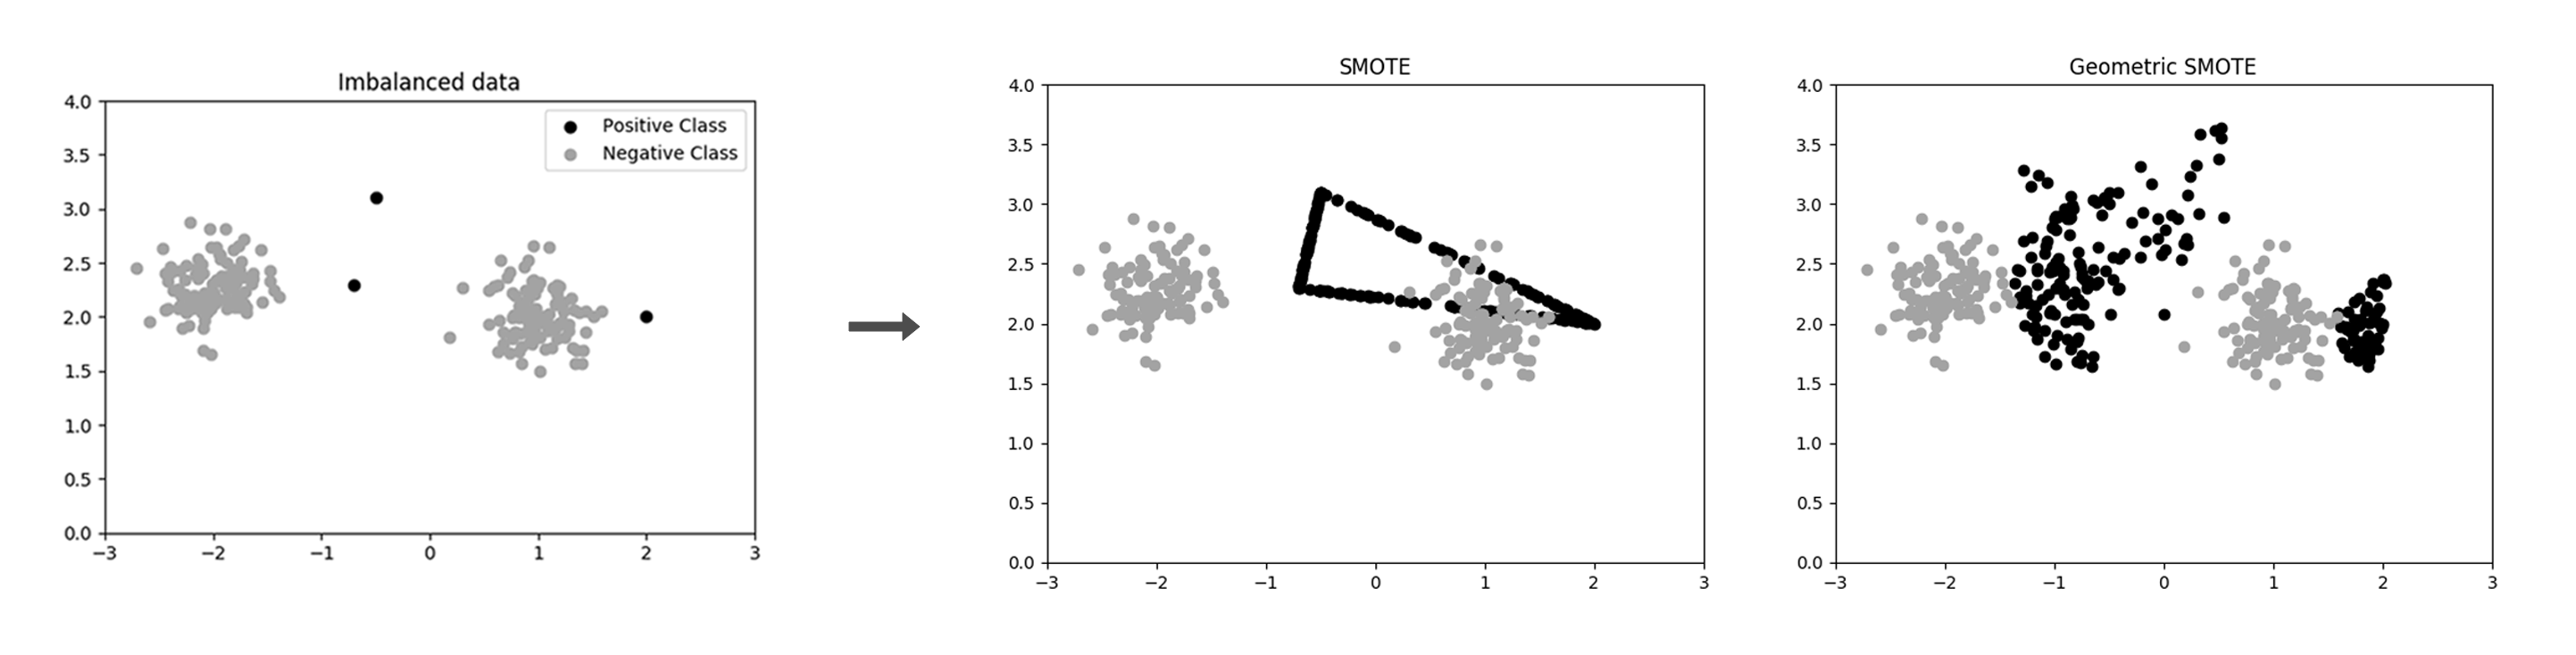
\includegraphics[width=1\linewidth]{../analysis/smote_vs_gsmote}
	\caption{Three positive class instances are used by SMOTE and G-SMOTE 
	to generate synthetic data. G-SMOTE generates non-noisy samples 
	with higher variety than SMOTE.}
	\label{fig:smotevsgsmote}
\end{figure}

The experimental study of \cite{Douzas.2019} includes an extensive comparison
between G-SMOTE and SMOTE using 69 imbalanced datasets and several classifiers.
The results show that G-SMOTE outperforms SMOTE, Random Oversampling and the
case of no over-sampling, across all datasets, classifiers and performance
metrics.

\section{Proposed method}

In the following section, we present G-SMOTE as a novel data generation
procedure for small datasets in the case of binary classification. Originally
developed for the imbalanced learning problem, we adapt the algorithm to not
only re-sample the minority class, but the entire dataset independent from the
class distribution. 

\subsection{G-SMOTE algorithm}

As mentioned above, the G-SMOTE algorithm randomly generates artificial data
within a geometrical region of the input space. The size of this area is derived
from the distance of the selected sample to one of its nearest neighbors,
whereas the shape is determined by the hyper-parameters called
\textit{truncation factor} and \textit{deformation factor}. Additionally, the
\textit{selection strategy} hyper-parameter  of G-SMOTE modifies the standard
SMOTE selection process and also affects the size of the geometric region.
Although the main concept can be adapted from the original method to the small
dataset problem, the \textit{selection strategy} requires some minor adjustments
which will be described hereafter.

In what follows, G-SMOTE is applied to the case of binary classification tasks
with the objective to generate artificial data for both classes, called
arbitrarily the positive and negative class. The application for the multi-class
case is also straightforward and it is based on the binarization of the problem
through the one-vs-all approach. Finally, regression tasks require an extensive
modification of the original G-SMOTE algorithm and they will be a topic of
future research.

\subsection{Adapted G-SMOTE algorithm}

The inputs of the G-SMOTE algorithm are the positive and negative class samples
\( S_{pos} \), \( S_{neg} \) respectively, the three geometric hyper-parameters
\textit{truncation factor}, \textit{deformation factor} and \textit{selection
strategy} as well as the number of generated samples for the positive class
\(N_{pos} \) and for the negative class \( N_{neg} \). A sensible choice for the
last two inputs, used also in the experimental procedure below, is to preserve
the class distribution in the re-sampled dataset. The adapted G-SMOTE algorithm
can be generally described in the following steps:

\begin{enumerate}

\renewcommand{\labelenumii}{\theenumii}
\renewcommand{\theenumii}{\theenumi.\arabic{enumii}.}

	\item An empty set \( S_{gen} \) is initialized. \( S_{gen} \) will be
	populated with artificial data from both classes.

	\item \( S_{pos} \) is shuffled and the process described below is repeated
	\( N_{pos} \) times until \( N_{pos} \) artificial points have been
	generated.

	\begin{enumerate}

		\item A positive class instance \( \textbf{x}_{center} \) is selected
		randomly from as \( N_{pos} \) the center of the geometric region.

		\item Depending on the values of \( \alpha_{sel} \) \( (positive,
		negative \) or \( combined) \), this step results in a randomly selected
		sample \(\textbf{x}_{surface} \) which belongs to either \( S_{pos} \)
		or \( S_{neg} \).

		\item A random point \(\textbf{x}_{gen} \) is generated inside the
		hyper-spheroid centered at \( \textbf{x}_{center} \). The major axis of
		the hyper-spheroid is defined by \( \textbf{x}_{surface} -
		\textbf{x}_{center} \) while the permissible data generation area as
		well as the rest of geometric characteristics are determined by the
		hyper-parameters \textit{truncation factor} and \textit{deformation
		factor}.

		\item \( \textbf{x}_{gen} \) is added to the set of generated samples
		\( \textbf{S}_{gen} \).
	
	\end{enumerate}

	\item Step 2 is repeated using the substitution \( pos \leftrightarrow neg
	\) until \( N_{neg} \) artificial points have been generated.

\end{enumerate}

Therefore, the adapted G-SMOTE algorithm applies independently the original
G-SMOTE algorithm for both the positive and negative class. The above
description of the algorithm excludes mathematical formulas and details which
can be found in \cite{Douzas.2019}. Figure \ref{fig:gsmotemechanism} shows an
example of the adapted G-SMOTE data generation process for the three different
values of the \textit{selection strategy} hyper-parameter when positive class
data generation is considered.

\begin{figure}[H]
	\centering
	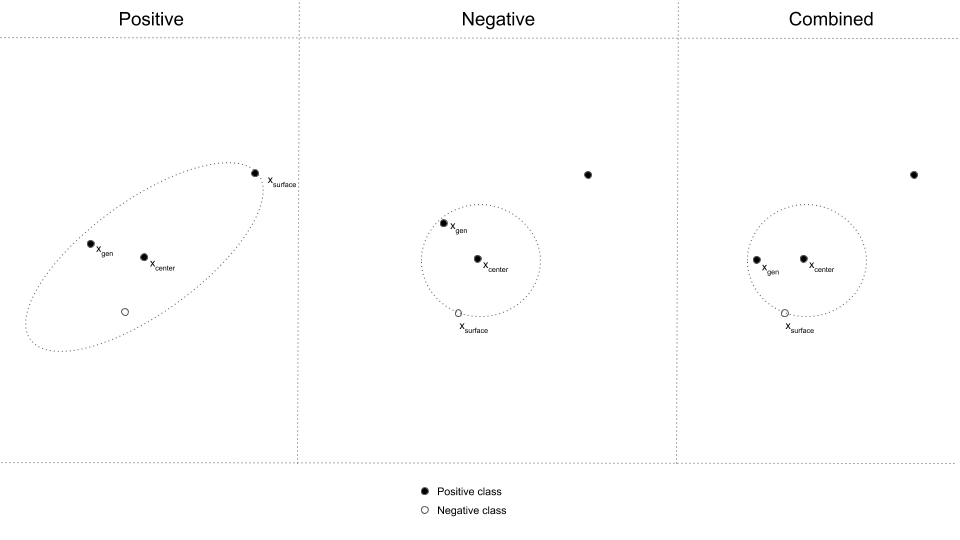
\includegraphics[width=1\linewidth]{../analysis/smote_mechanism.png}
	\caption{Three positive class instances are used by SMOTE and G-SMOTE 
	to generate synthetic data. G-SMOTE generates non-noisy samples 
	with higher variety than SMOTE.}
	\label{fig:gsmotemechanism}
\end{figure}

\section{Research methodology}

The main objective of this work is to compare G-SMOTE with other over-sampling
techniques when it comes to the small dataset problem. Therefore, we use a
variety of datasets, evaluation measures and classifiers to evaluate the
performance of over-samplers. A description of this set-up, the experimental
procedure as well as the software implementation is provided in this section.

\subsection{Experimental data}

Ten datasets are used to test the performance of G-SMOTE which are retrieved
from UCI Machine Learning Repository \cite{Dua.2019}. The focus on the selection
of the data lies on binary classification problems with a balanced distribution
of the two classes. In order to assure generalizability of the results, the
datasets include different topics such as health care, finance, business and
physics as well as different sample sizes. Details of the datasets are presented
in the following table:

\begin{longtable}{llll}
	\specialrule{.1em}{.05em}{.05em}
	\textbf{Dataset} & \textbf{Number of samples} & \textbf{Number of
	attributes} & \textbf{Area} \\
	\hline
	Arcene & 900 & 10.000 & Health Care \\
	Audit & 776 & 18 & Business \\
	Banknote Authentication & 1.372 & 5 & Finance \\
	Spambase & 4.610 & 57 & Business\\
	Breast Cancer & 699 & 10 & Health Care\\
	Indian Liver Patient & 583 & 10 & Health Care\\
	Ionosphere & 351 & 34 & Physics\\
	MAGIC Gamma Telescope & 19.020 & 11 & Physics\\
	Musk & 6.598 & 168 & Physics\\
	Parkinsons & 197 & 23 & Health Care\\
	\specialrule{.1em}{.05em}{.05em}
\caption{\label{tab:datasets}Description of the datasets} 
\end{longtable}

\subsection{Evaluation measures}

To evaluate the performance of G-SMOTE, the experiment includes two different
measures. First, \textit{Accuracy} is used as one of the most common metrics for
evaluating classification models \cite{M.2015}. \textit{Accuracy} measures the
ratio of correct predictions over the total number of instances. The
mathematical formula is the following:

$$ \textit{Accuracy} = \frac{TP + TN}{TP +TN + FP + FN}$$

where \( TP \), \( TN \) denote the number of correctly classified positive and
negative instances respectively while \(FP \), \( FN\) denote the number of
misclassified negative and positive instances, respectively. The
\textit{Accuracy} metric might be inappropriate for datasets with a significant
difference between the number of positive and negative classes since rare
classes have a small impact to the final outcome compared to the majority
classes. To make sure the contribution in the accuracies of the two classes stay
relatively balanced, we include the geometric mean score (\textit{G-Mean}) as a
second measure. \textit{G-Mean} is the geometric mean of \textit{sensitivity}
and \textit{specificity}:

$$\textit{G-Mean} = \sqrt{sensitivity \times specificity} = \sqrt{\dfrac{TP}{TP + FN}
\times \dfrac{TN}{TN + FP}}$$

\subsection{Machine learning algorithms}

The experiment is conducted with several classifiers. We use the following four
algorithms: Logistic Regression (LR) \cite{McCullagh.2019}, K-Nearest Neighbors
(KNN) \cite{Cover.1967}, Decision Tree (DT) \cite{Salzberg.1994} and Gradient
Boosting (GB) \cite{Friedman.2001}.

\subsection{Experimental procedure}

The main concept of the experimental procedure is to reduce the size of the
datasets presented in table \ref{tab:datasets}, increase their size artificially
back to the initial using different over-samplers and compare the results with
the original dataset which is considered to be the benchmark. This method allows
us to directly compare the quality of the artificially generated samples to the
observed data. In order to evaluate if the proposed method can improve
artificial data generation, we compare G-SMOTE with SMOTE, Borderline SMOTE and
Random Oversampling. Also, we apply the machine learning algorithms to the
under-sampled data with the objective to assess their performance with a smaller
amount of data. To under-sample the data we use a ratio of 50, 75, 90 and 95
percent of the original dataset. For example, with an undersampling ratio of 95
percent, we take only five percent of the original data as a base to apply the
over-sampling mechanism. This approach aims to provide an understanding of the
classification performance as the size of the dataset diminishes.

Figure \ref{fig:experimentalprocedure} visualizes the experimental process: 

\begin{figure}[H]
	\centering
	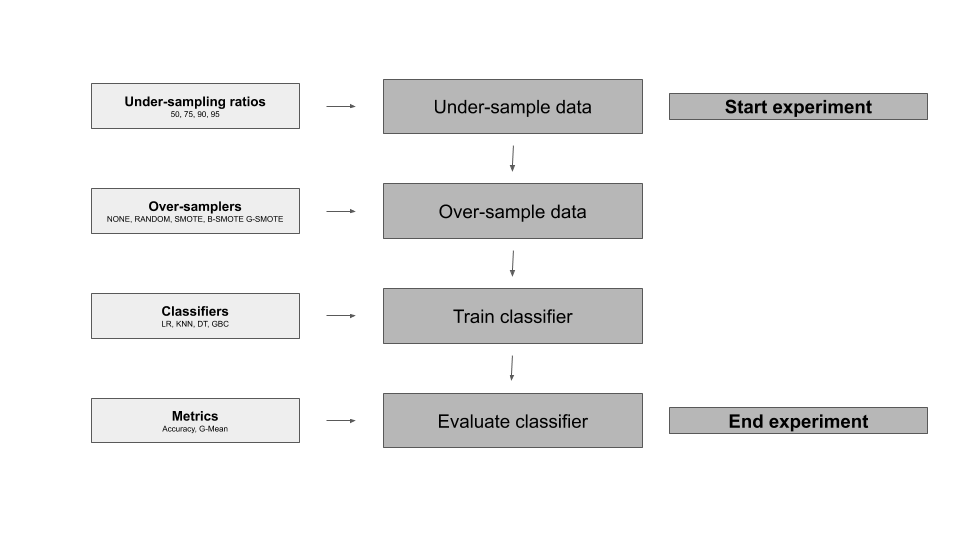
\includegraphics[width=0.7\linewidth]{../analysis/experimental_procedure.png}
	\caption{High-level experimental procedure}
	\label{fig:experimentalprocedure}
\end{figure}

We use \( k \)-fold cross-validation scores with \( k = 5 \) to assess the
performance of the models for each combination of over-sampler and classifier.
The dataset \( D \) is randomly split into \( k \) subsets (folds) \( D_1, D_2,
… D_k \) of approximately equal size. Each fold is used as a validation set and
the remaining folds are used to train the model with \( k \) iterations. This
procedure is repeated until each \( k \) have been used as a validation set
\cite{Han.2012}. Based on the above description, the experiment is conducted in
the following steps within one iteration:

\begin{enumerate}
	
	\item 
	Split the dataset into \( k \)-fold cross-validation sets.

	\item 
	Under-sample \( k - 1 \) folds such that the class frequency remains 
	the same as the original with a ratio of 50, 75, 90 and 95 percent.

	\item 
	Over-sample \( k - 1 \) folds to the original size of the
	dataset (class ratio remains the same) with G-SMOTE, SMOTE, Borderline
	SMOTE, Random Oversampling. Also include the no oversampling case.

	\item 
	Train the model with the classifiers LR, KNN, DT and GB

	\item 
	Test the model with the remaining, original fold

\end{enumerate}	

This procedure is repeated 3 times and the highest cross validation score for
each combination of dataset, classifier, oversampler and evaluation metric is
reported.

In order to confirm the statistical significance of the experimental results,
the Friedman test \cite{Sheldon.1996} as well as the Holm test
\cite{JanezDemsar.2006} are applied. Ranking scores are assigned to each
over-sampling method with scores of 1 to 5 for the best and worst performing
methods, respectively. The Friedman test is a non-parametric procedure that
compares the average rankings of the algorithms under the null hypothesis that
all show identical performance independent of the selected classifier and
evaluation metric. If the null-hypothesis is rejected to our favor, we proceed
with the Holm test. The Holm test acts as a post-hoc test for the Friedman test
for controlling the family-wise error rate when all algorithms are compared to a
control method. It is a powerful non-parametric test in situations where we want
to test whether a newly proposed method is better than existing ones. The
control method in our case is the proposed G-SMOTE method and is tested under
the null hypothesis that it performs similarly to the rest of over-samplers for
every combination of classifier and metric.

\subsection{Software Implementation}

The implementation of the experimental procedure is based on Python programming
language using the Scikit-Learn library
\cite{PedregosaF.VaroquauxG.GramfortA.MichelV.ThirionB.GriselO.BlondelM.Prette.2011}.
All functions, algorithms, experiments and results reported are provided at
\url{https://github.com/AlgoWit/publications/tree/master/small-data-oversampling}.
Additionally, Research-Learn library
(\url{https://github.com/AlgoWit/research-learn}) provides a framework to
implement comparative experiments, being also fully integrated with the
Scikit-Learn ecosystem.

\section{Results and discussion}

In this section the performance of the different oversamplers and the results 
of the statistical tests are presented and analyzed.

\subsection{Comparative presentation}

The mean cross validation scores and the standard error per classifier and
metric across all datasets are presented in Table \ref{tab:mean_sem_scores}. The
scores are presented for each under-sampling ratio to evaluate how the methods
perform as the dataset size diminishes. We include the benchmark method that
represents the original dataset without applying under-sampling before training
the algorithm. This sample set is seen as the ground truth of our experiments
which is expected to obtain the best results by design.

\begin{center}
\begin{footnotesize}
\csvreader[
	longtable=lllllllll,
	table head=
	\toprule\mdseries Ratio & \mdseries Classifier & \mdseries Metric & \mdseries NONE & \mdseries 
	RANDOM & \mdseries SMOTE & \mdseries B-SMOTE & \mdseries G-SMOTE & \mdseries BENCHMARK \\
	\midrule\endhead
	\bottomrule\endfoot,
	late after line=\\,
	before reading={\catcode`\#12},
	after reading={\catcode`\#12},
	]{../analysis/mean_sem_scores.csv}
	{1=\ratio,2=\classifier,3=\metric,4=\none,5=\random,6=\smote,7=\bsmote,
		8=\gsmote,9=\benchmark}
	{\ratio & \classifier & \metric & \none & \random & \smote & \bsmote & 	
	\gsmote & \benchmark}
\end{footnotesize}
\addtocounter{table}{-1}
\captionof{table}{Results for mean cross validation 
	scores of oversamplers (NONE corresponds to No Oversampling, RANDOM 
	to Random Oversampling and B-SMOTE to Borderline SMOTE)}
\label{tab:mean_sem_scores}
\end{center}

This table shows that G-SMOTE outperforms all over-sampling methods almost for
all combinations of classifiers and metrics. Throughout the scores we can
observe that all over-samplers have a better performance as the dataset increase
their size i.e. the under-sampling ratio gets smaller.  Particularly, the scores
of G-SMOTE are the closest to the ones of the Benchmark method which implies
that the proposed method is able to artificially establish a representative
dataset.

Table \ref{tab:mean_sem_perc_diff_scores} presents the mean and standard error
of percentage difference between G-SMOTE and No Oversampling. It shows that
G-SMOTE performs significantly better compared to the case where no
over-sampling is applied in every combination of under-sampling ratio,
classifier and metric. Particularly, the performance gap increases for higher
under-sampling ratios.

\begin{center}
	\begin{footnotesize}
		\csvreader[
		longtable=llll,
		table head=
		\toprule\mdseries Ratio & \mdseries Classifier & \mdseries Metric & \mdseries \% Difference \\
		\midrule\endhead
		\bottomrule\endfoot,
		late after line=\\,
		before reading={\catcode`\#12},
		after reading={\catcode`\#12},
		]{../analysis/mean_sem_perc_diff_scores.csv}
		{1=\ratio,2=\classifier,3=\metric,4=\difference}
		{\ratio & \classifier & \metric & \difference}
	\end{footnotesize}
	\addtocounter{table}{-1}
	\captionof{table}{Results for percentage difference between G-SMOTE and SMOTE}
	\label{tab:mean_sem_perc_diff_scores}
\end{center}

As explained in section 4, a ranking score in the range 1 to 5 is assigned to
each oversampler. The mean ranking of all oversampling methods across the
datasets is presented in the following figure: 

\begin{figure}[H]
	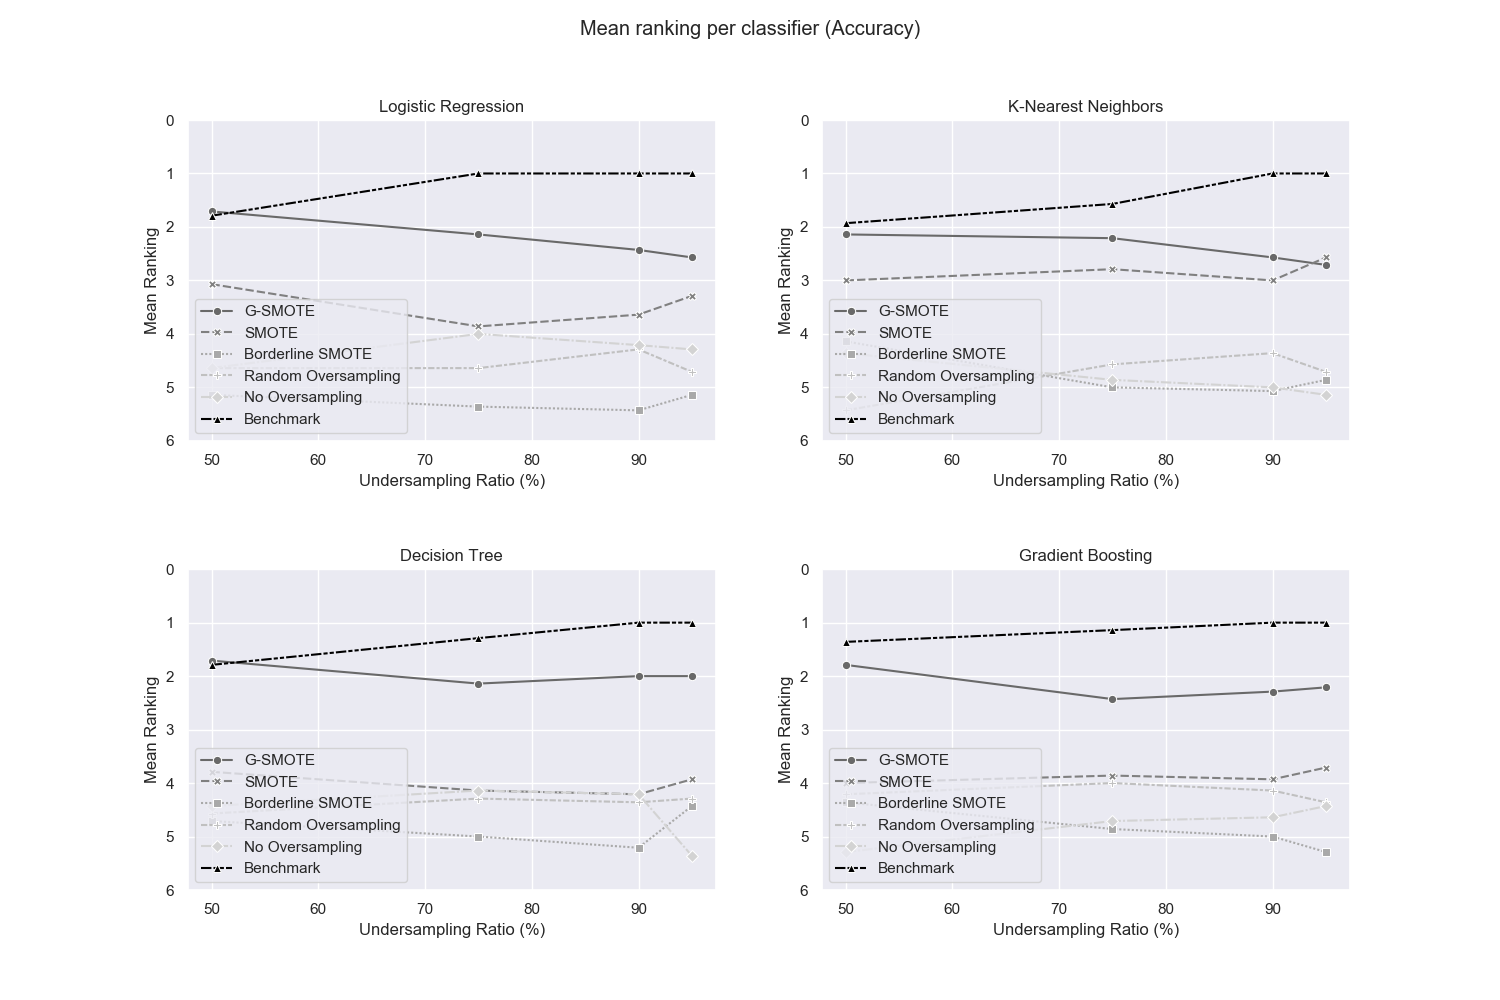
\includegraphics[width=1\linewidth]
		{../analysis/mean_ranking_per_classifier_accuracy}
	\caption{Mean ranking per classifier (Accuracy)}
	\label{fig:mean_ranking_per_classifier_accuracy}
\end{figure}

Looking at the graphs, G-SMOTE is ranked on the top place when comparing with
SMOTE, Borderline SMOTE, Random Oversampling and No Oversampling. Additionally,
G-SMOTE slightly outperforms the Benchmark method using the classifiers Logistic
Regression and Decision Tree in the mean ranking. 

\subsection{Statistical Analysis}

To confirm the significance of the above presented results we apply the Friedman
test as well as the Holm Test on the above results. The application of the
Friedman test is presented below:

\begin{center}
	\begin{footnotesize}
		\csvreader[
		longtable=llll,
		table head=
		\toprule\mdseries Classifier & \mdseries Metric & \mdseries p-value & 
		\mdseries Significance \\
		\midrule\endhead
		\bottomrule\endfoot,
		late after line=\\,
		before reading={\catcode`\#12},
		after reading={\catcode`\#12},
		]{../analysis/friedman_test.csv}
		{1=\classifier,2=\metric,3=\pvalue,4=\significance}
		{\classifier & \metric & \pvalue & \significance}
	\end{footnotesize}
	\addtocounter{table}{-1}
	\captionof{table}{Results for Friedman test}
	\label{tab:friedman_test.csv}
\end{center}

Therefore, the null hypothesis of the Friedman test is rejected at a 
significance level of a = 0.05, i.e. the over-samplers do not perform similarly 
in the mean rankings for any combination of classifier and evaluation metric.

The Holm's method is applied to adjust the $\text{p-values}$ of the paired 
difference test with G-SMOTE algorithm as the control method. The results are 
shown in table \ref{tab:holm_test}:

\begin{center}
	\begin{footnotesize}
		\csvreader[
		longtable=llllll,
		table head=
		\toprule\mdseries Classifier & \mdseries Metric & \mdseries NONE & 
		\mdseries RANDOM & \mdseries SMOTE & \mdseries B-SMOTE\\
		\midrule\endhead
		\bottomrule\endfoot,
		late after line=\\,
		before reading={\catcode`\#12},
		after reading={\catcode`\#12},
		]{../analysis/holms_test.csv}
		{1=\classifier,2=\metric,3=\none,4=\random,5=\smote,6=\bsmote}
		{\classifier & \metric & \none & \random & \smote & \bsmote}
	\end{footnotesize}
	\addtocounter{table}{-1}
	\captionof{table}{Adjusted $\text{p-values}$ using Holm test (B-SMOTE 
	corresponds to Borderline 
	SMOTE)}
	\label{tab:holm_test}
\end{center}

At a significance level of a = 0.05 the null hypothesis of the Holm's test is
rejected for 25 out 32 combinations. This indicates that the proposed method
outperforms all other methods in most cases.  

\section{Conclusions}

This paper illustrates an effective solution to mitigate the small dataset
problem in binary classification tasks. As shown above, the over-sampling
algorithm G-SMOTE has the ability to generate high quality artificial samples
and improve the prediction accuracy of the classifiers used in the experiments.
This improvement relates to its capability of increasing the diversity of new
instances while avoiding the generation of noisy samples. An important point is
that G-SMOTE significantly improves classification performance compared to the
case where only the small data are used. Also G-SMOTE outperforms standard
over-sampling approaches such as Random Over-Sampling and SMOTE, being closer to
the benchmark scores than any of them. Finally, G-SMOTE implementation is
available on (\url{https://github.com/AlgoWit/geometric-smote}).

\bibliography{references}
\bibliographystyle{apalike}

\end{document}
